\chapter{Kubernetes}
In this chapter, we will briefly describe Kubernetes technology, which has been used as the foundation for local solutions studied in recent years. This thesis integrates Kubernetes with Liqo technology.

As stated in its official documentation~\cite{k0-1}, Kubernetes is a portable, extensible, open source platform for managing containerized workloads and services, that facilitates both declarative configuration and automation. Kubernetes emerged as a platform designed to automate the management of containerized applications, ensuring periodic checks to maintain alignment between the actual operational state and the defined ideal state through a declarative language. 

A decade since its release as an open-source project, Kubernetes stands as one of the most extensively utilized platforms worldwide. This project focuses on k3s, a lightweight variant of Kubernetes tailored for operation in resource-constrained environments.

\section{Basic concepts}
The foundational principles underlying the architecture of Kubernetes are articulated as follows:
\begin{enumerate}
\item Implementation-agnostic APIs: Each Kubernetes object can be implemented differently depending on the version being used, yet the interface used to manage these objects remains consistent across all versions.
\item Completely declarative specification: Kubernetes facilitates the use of a declarative language instead of the traditional imperative approach, simplifying application management by specifying the desired state directly rather than detailing how to achieve that state from various starting points.
\item Control loop-oriented approach: Kubernetes employs components known as controllers that cyclically monitor whether the current state aligns with the desired state. If discrepancies are identified, these controllers initiate actions to minimize the gap between the states. This behaviour is shown in Figure~\ref{fig:loop2}.
\end{enumerate}

\begin{figure}[ht]\centering
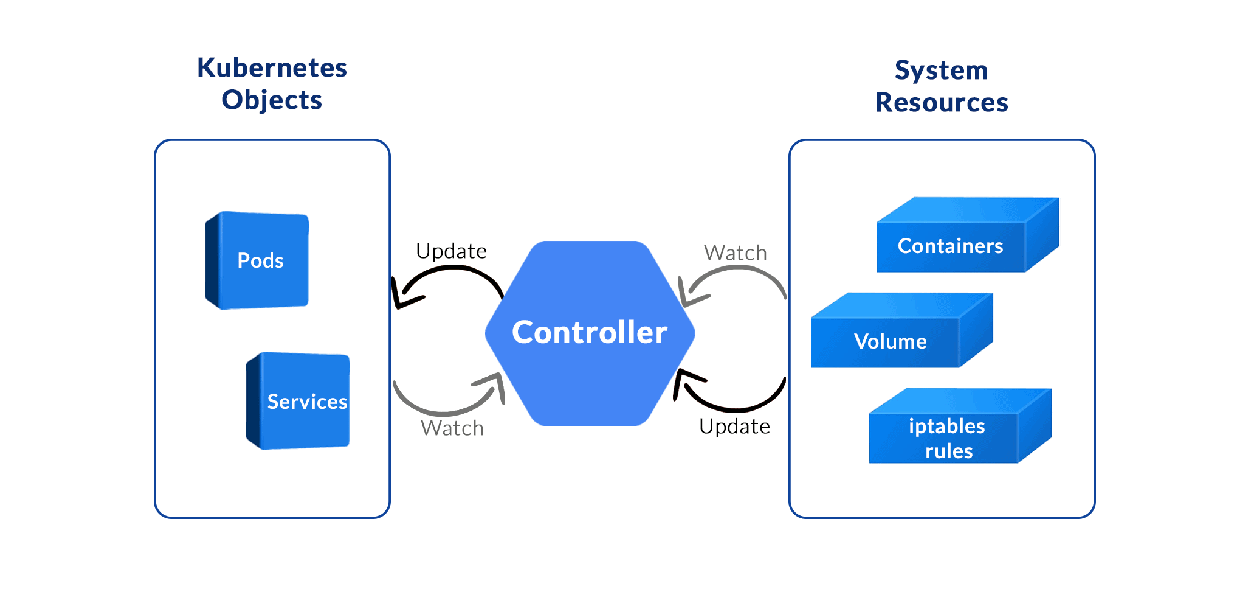
\includegraphics[scale=0.7]{Pictures/loop}
\caption[Control loop mechanism]{Control loop mechanism\footnotemark.}\label{fig:loop2}
\end{figure}

These principles are the cornerstone of Kubernetes, facilitating efficient management and orchestration of containerized applications in a variety of computing environments.

\footnotetext{\url{https://k21academy.com/docker-kubernetes/kubernetes-operator/}}

Every object within Kubernetes is meticulously crafted to adhere to foundational principles, starting with its smallest operational unit: the object Pod. A Pod may consist of one or more containers that will run the application and its configuration is defined in its respective YAML file. This file may reference other configuration files using key-value pairs, such as Secrets or ConfigMaps, useful in case these configurations are repeated multiple times. 

Containers within pods typically share a common network and can communicate with each other by default. However, Kubernetes provides flexibility to configure additional sharing capabilities, including interactions with the underlying host infrastructure, depending on specific deployment requirements. In addition to application containers, a od can include init containers that execute during the Pod's startup phase to set up the environment. Kubernetes also supports the injection of ephemeral containers for debugging purposes while a Pod is running. In typical usage scenarios, direct interaction with Pods is uncommon, as they are ephemeral entities within Kubernetes. Instead, management typically focuses on higher-level objects such as controllers. The emphasis is on the collective state of these replicas rather than individual Pods. 

Pods are typically instantiated and taked care through the implementation of various Kubernetes controllers. The Deployment controller, commonly used for stateless applications, describes the desired application state while managing scalability through the ReplicaSet. For stateful applications, the StatefulSet controller is normally utilized, managing the Pod-to-volume binding and ensuring properties such as unique network IDs that the stateful application required to function properly. A DaemonSet places a replica of a Pod on each node that matches its nodeSelector options (or on every node in the cluster if nodeSelector is not set). 

As a controller, this behavior supports dynamic changes: if a node is added to the network, the DaemonSet starts a Pod replica on that node; if a node is removed, the corresponding pod is not rescheduled. Typically, DaemonSets are employed for specific tasks such as log collection and node monitoring.

While controllers oversee the lifecycle of Pods, Pod discovery is entrusted to Services. These Kubernetes objects target all pods matching their selector criteria, facilitating exposure both within and outside the cluster. ClusterIP services expose pods solely within the cluster, whereas NodePort or LoadBalancer services extend pod accessibility externally.

Pods are instantiated on physical or virtual machines known as nodes, which serve either as master or worker nodes based on their role. A master node not only executes various Kubernetes components, as previously discussed, but also hosts the cluster's control plane such as the scheduler, controller manager, and API server. Conversely, a worker node is dedicated solely to executing the workloads of Kubernetes objects.

The cluster, comprising these nodes, can be structured as a single-master or multi-master configuration. In a multi-master setup, control plane components are replicated across all master nodes, and decisions are made via a consensus mechanism facilitated by the etcd quorum process, which utilizes the Raft algorithm~\cite{k1-1}.  This setup necessitates an odd number of master nodes to prevent split-brain~\cite{k1-2} scenarios and reduce decision-making delays. 

These structural and operational principles form the backbone of Kubernetes architecture, facilitating scalable and efficient container orchestration in diverse computing environments.

\section{K3s}
K3s is a lightweight variant of Kubernetes tailored for operation in resource-constrained environments,  as described in the official documentation\cite{k2-1}:
\begin{itemize}
\item Edge
\item Homelab
\item Internet of Things (IoT)
\item Continuous Integration (CI)
\item Development
\item Single board computers (ARM)
\item Air-gapped environments
\item Embedded K8s
\item And as the official page says, situations where a PhD in K8s clusterology is infeasible
\end{itemize}
K3s efficiently utilizes approximately half the memory resources compared to Kubernetes (K8s) by implementing several optimizations. These include eliminating legacy libraries, opting for lightweight alternatives such as SQLite instead of the standard etcd for database management, and containerd instead of Docker as the container runtime. Additionally, internal mechanisms have been adjusted to reduce memory consumption.

K3s gets its name from the fact that it uses about half the memory, hence it was jokingly named K3s as it consists of 5 letters(K+3+s), which is half of the 10 letters in Kubernetes(K+8+s).

This was demonstrated by two researchers in 2021, Sebastian Böhm and Guido Wirtz~\cite{k2-1}. In their tests, they compared the standard Kubernetes technologies, K3s, and microk8s, using 4 virtual machines with the following parameters

\begin{itemize}
\item \textbf{CPU:} 2 vCPUs
\item \textbf{RAM:} 4 GB memory
\item \textbf{Disk memory:} SSD with a capacity of 50GB
\item \textbf{OS:} Ubuntu 20.04
\end{itemize}

The results indicated that CPU and memory resource usage were quite similar across all three technologies, but k3s demonstrated significantly lower disk space utilization compared to the standard Kubernetes, approximately half as much, as illustrated in the Figure~\ref{fig:guido}.

\begin{figure}[ht]\centering
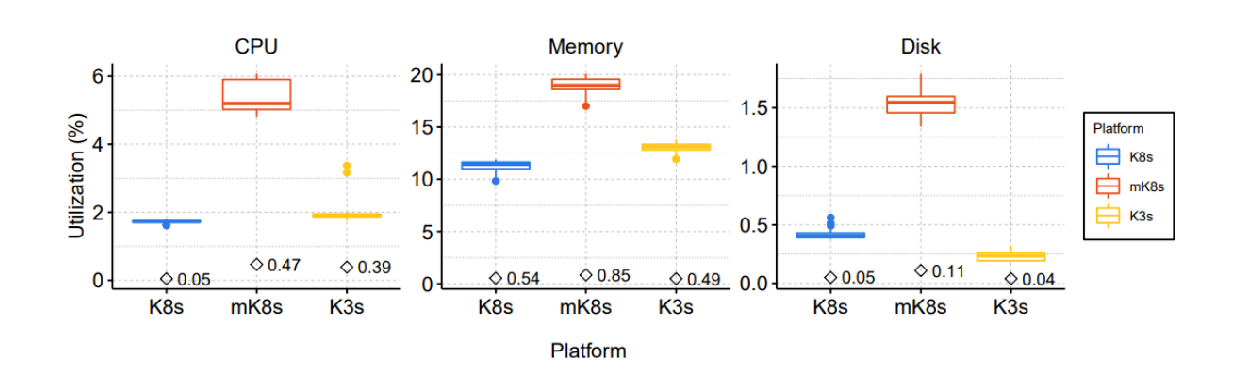
\includegraphics[scale=0.7]{Pictures/guido}
\caption{Resource utilization for K8s, MicroK8s, and K3s.}\label{fig:guido}
\end{figure}

The installation process is streamlined with a simple script that weighs less than 100 MB. Despite its compact size, this script effectively manages many of the complexities typically associated with Kubernetes environments, such as automatically configuring TLS certificates.

This revision clarifies the optimizations made in K3s to reduce memory usage and highlights the streamlined installation process while maintaining readability and technical accuracy.


